\documentclass{beamer}
\usetheme{Boadilla}
\usecolortheme{whale}

%\setbeamertemplate{headline}{}


\geometry{paperwidth=153mm,paperheight=86mm}  %* 16:10
%\geometry{paperwidth=96mm,paperheight=72mm}   %* 4:3



\usepackage[utf8x]{inputenc}
%\usepackage[spanish]{babel}

\usepackage{amsmath}
\usepackage{amsfonts}
\usepackage{amssymb}

\makeatletter
    \newenvironment{withoutheadline}{
        \setbeamertemplate{headline}[default]
        \def\beamer@entrycode{\vspace*{-\headheight}}
    }{}
\makeatother


\title[Bluetooth Low Energy]{Bluetooth Low Energy}
\author[BLE]{Juan Pablo Ruiz\\ 
\vspace{0.2cm}
{}}

\institute[]{
\includegraphics[width=0.1\textwidth]{./escudo.eps}}
\date{\today}



\begin{document}

\frame{% ===============================   START FRAME   ================================================
\maketitle
}% =====================================   END FRAME   ==========================================


\frame{% ===============================   START FRAME   ================================================
\frametitle{Bluetooth} 
Communication protocol for PC peripheral devices
\begin{center}
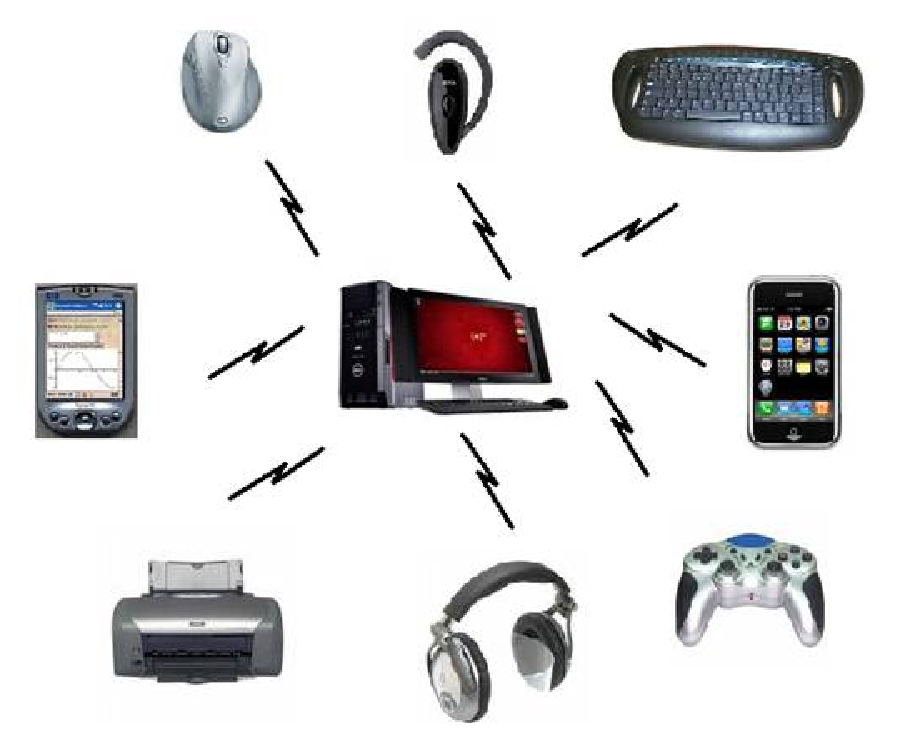
\includegraphics[width=0.5\textwidth]{./figures/blue1.eps}
\end{center}
}% =====================================   END FRAME   ==========================================

\frame{% ===============================   START FRAME   ================================================
\frametitle{Bluetooth and others evolution} 
More bandwidth, but one exception 
\begin{center}
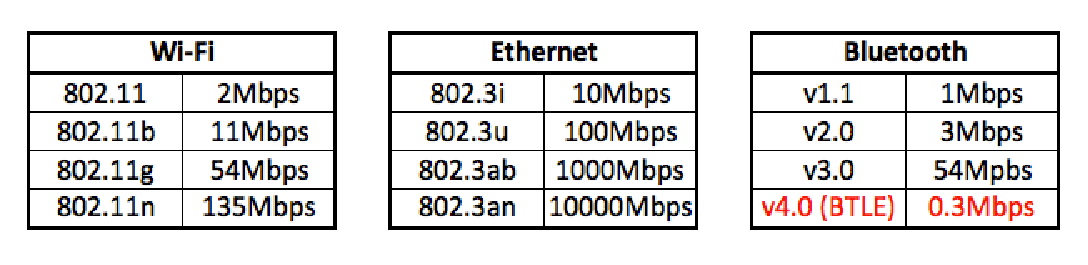
\includegraphics[width=0.9\textwidth]{./figures/rates.eps}
\end{center}
}% =====================================   END FRAME   ==========================================


\frame{% ===============================   START FRAME   ================================================
\frametitle{Bluetooth low energy} 
It’s good at small, discrete data transfers
\begin{center}
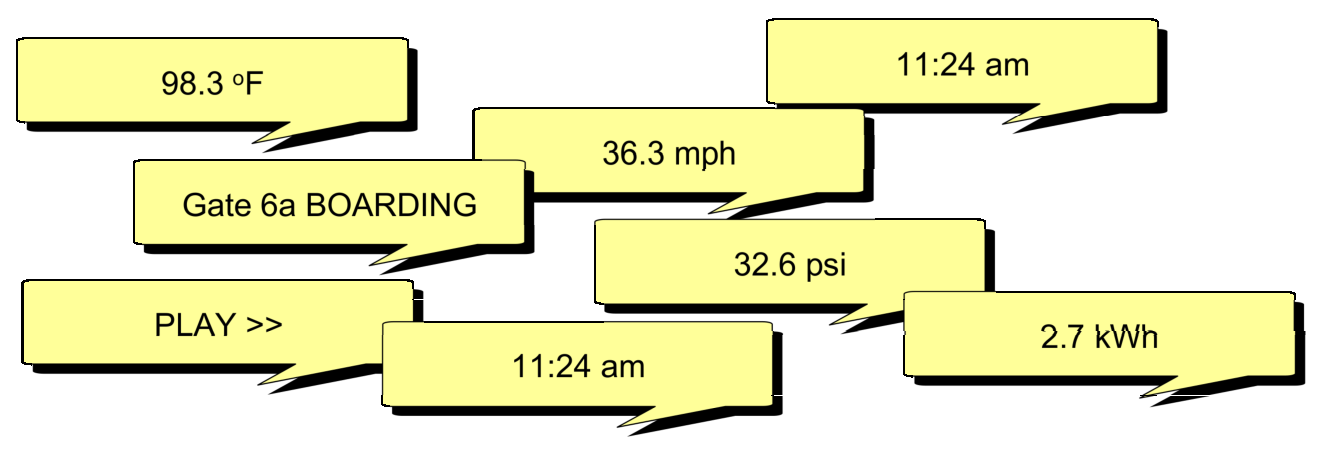
\includegraphics[width=0.9\textwidth]{./figures/data1.eps}
\end{center}
}% =====================================   END FRAME   ==========================================

\frame{% ===============================   START FRAME   ================================================
\frametitle{Bluetooth Low Energy} 
\begin{itemize}
\item A new radio, new protocol stack, new profile architecture and a new qualification regime \pause
\item It’s designed to run from coin cells \pause
\item New advertising mechanism, for ease of discovery \& connection \pause
\item Designed to be LOWEST cost and EASY to implement \pause
\item Very small silicon footprint and thereby very low cost \pause
\item Very secure through optional 128 bit AES encryption\pause
\item Very low power – designed to be asleep \pause
\end{itemize}
}% =====================================   END FRAME   ==========================================

\frame{% ===============================   START FRAME   ================================================
\frametitle{Bluetooth Low Energy} 
\begin{center}
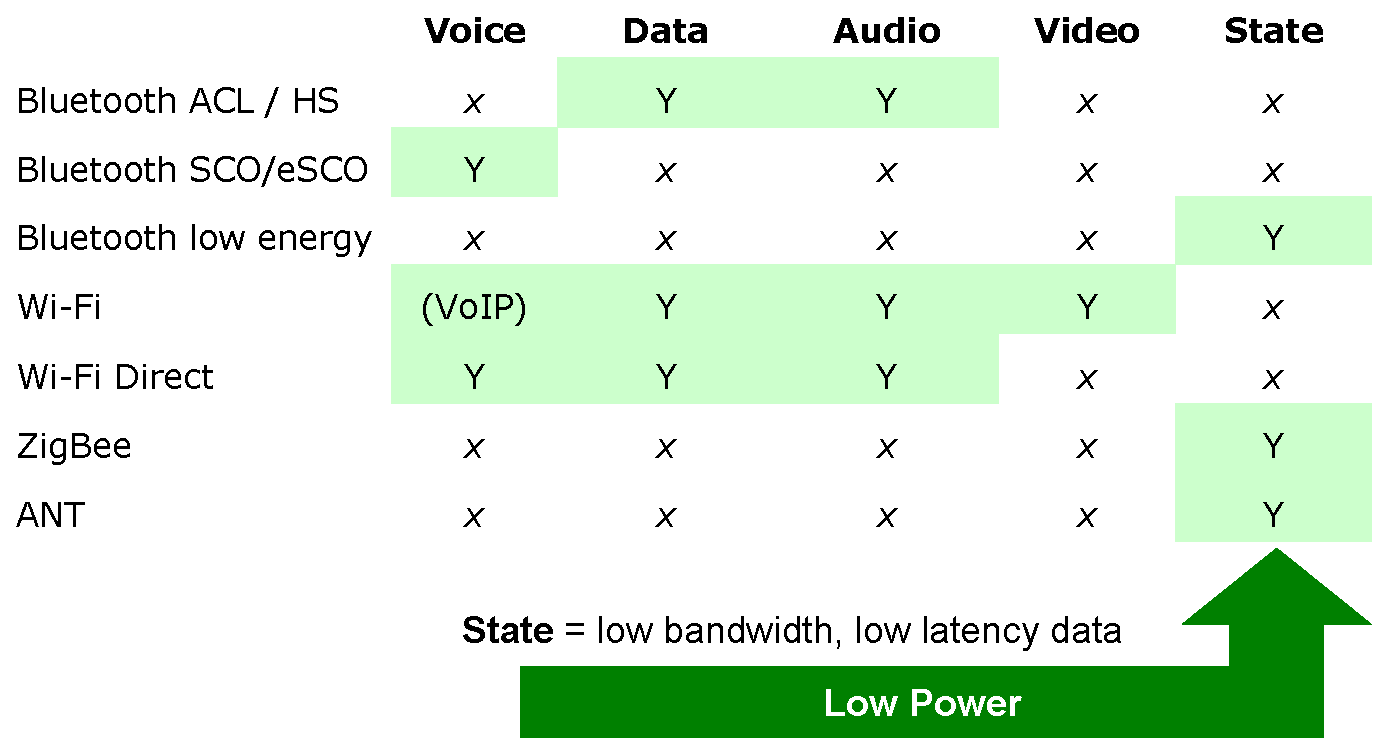
\includegraphics[width=0.7\textwidth]{./figures/comp1.eps}
\end{center}
}% =====================================   END FRAME   ==========================================

\frame{% ===============================   START FRAME   ================================================
\frametitle{Terminology - roles} 
\begin{itemize}
\item \textbf{Broadcaster:} Transmitter only
\item \textbf{Observer:} Receiver only
\item \textbf{Peripheral:} Supports slave role
\item \textbf{Central:}
\begin{itemize}
\item Supports master roles
\item Supports multiple connections
\item Initates connectfions to peripherals
\end{itemize}
\end{itemize}
Note: One device my support multiple roes
}% =====================================   END FRAME   ==========================================



\frame{% ===============================   START FRAME   ================================================
\frametitle{Bluetooth Low Energy} 
\begin{center}
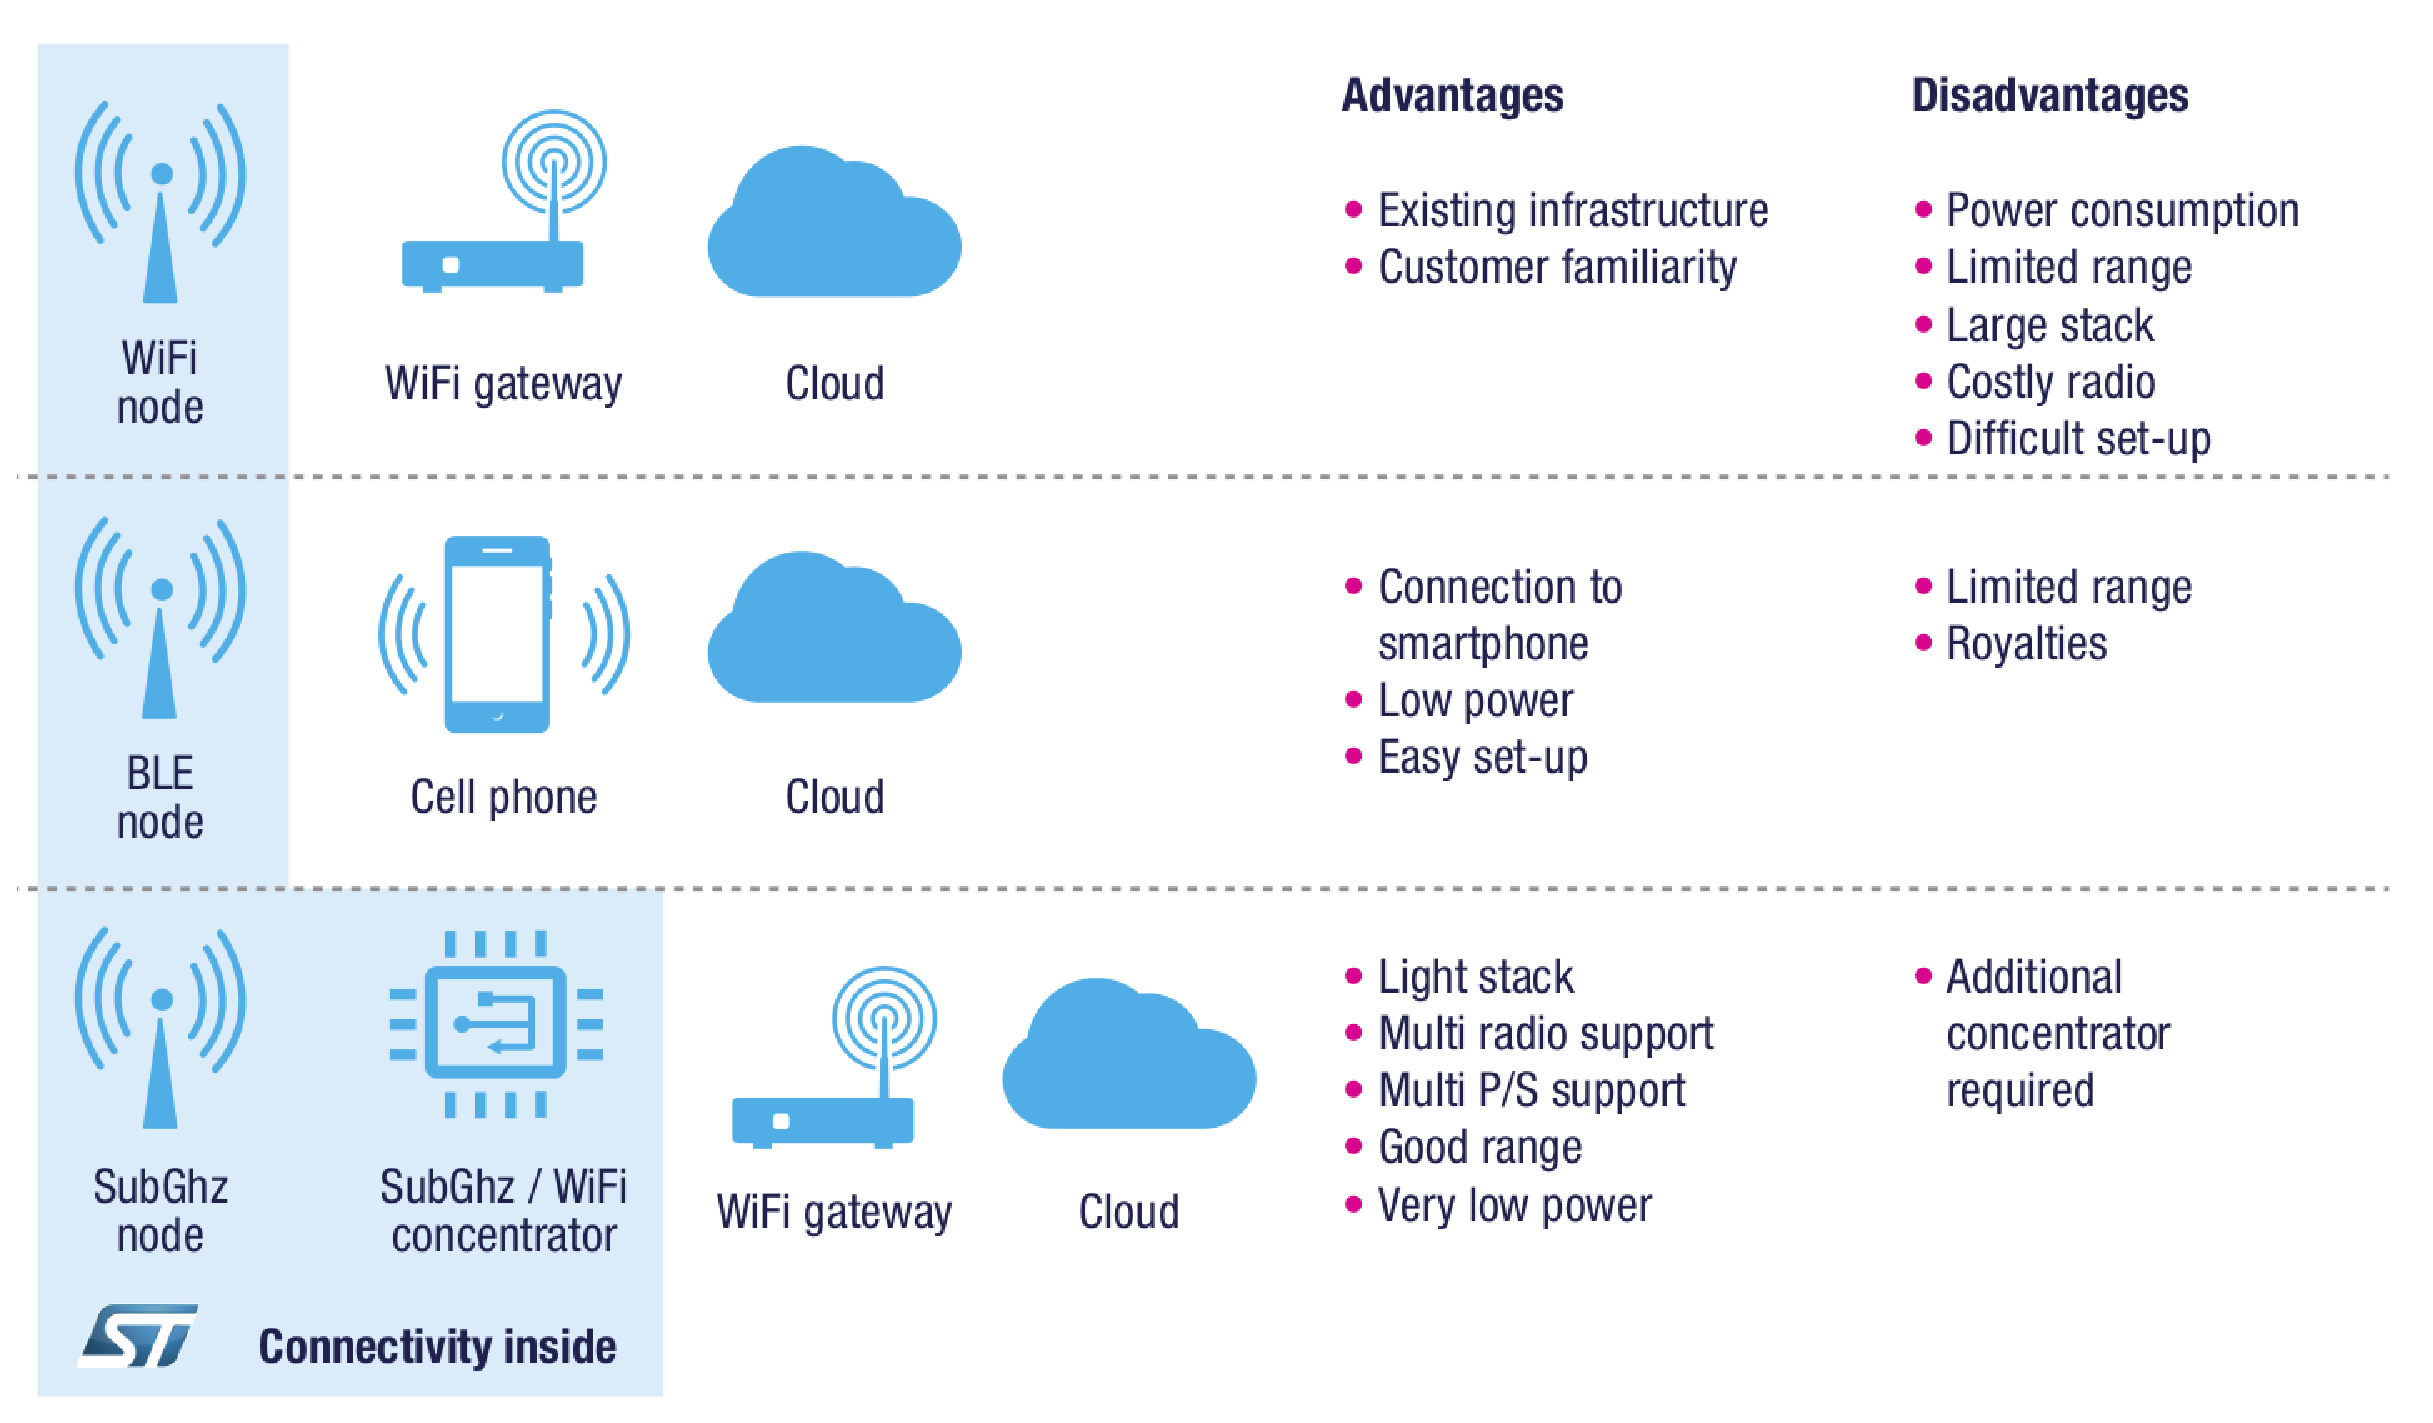
\includegraphics[width=0.7\textwidth]{./figures/comp2.eps}
\end{center}
}% =====================================   END FRAME   ==========================================

\frame{% ===============================   START FRAME   ================================================
\frametitle{Advertising} 
\begin{center}
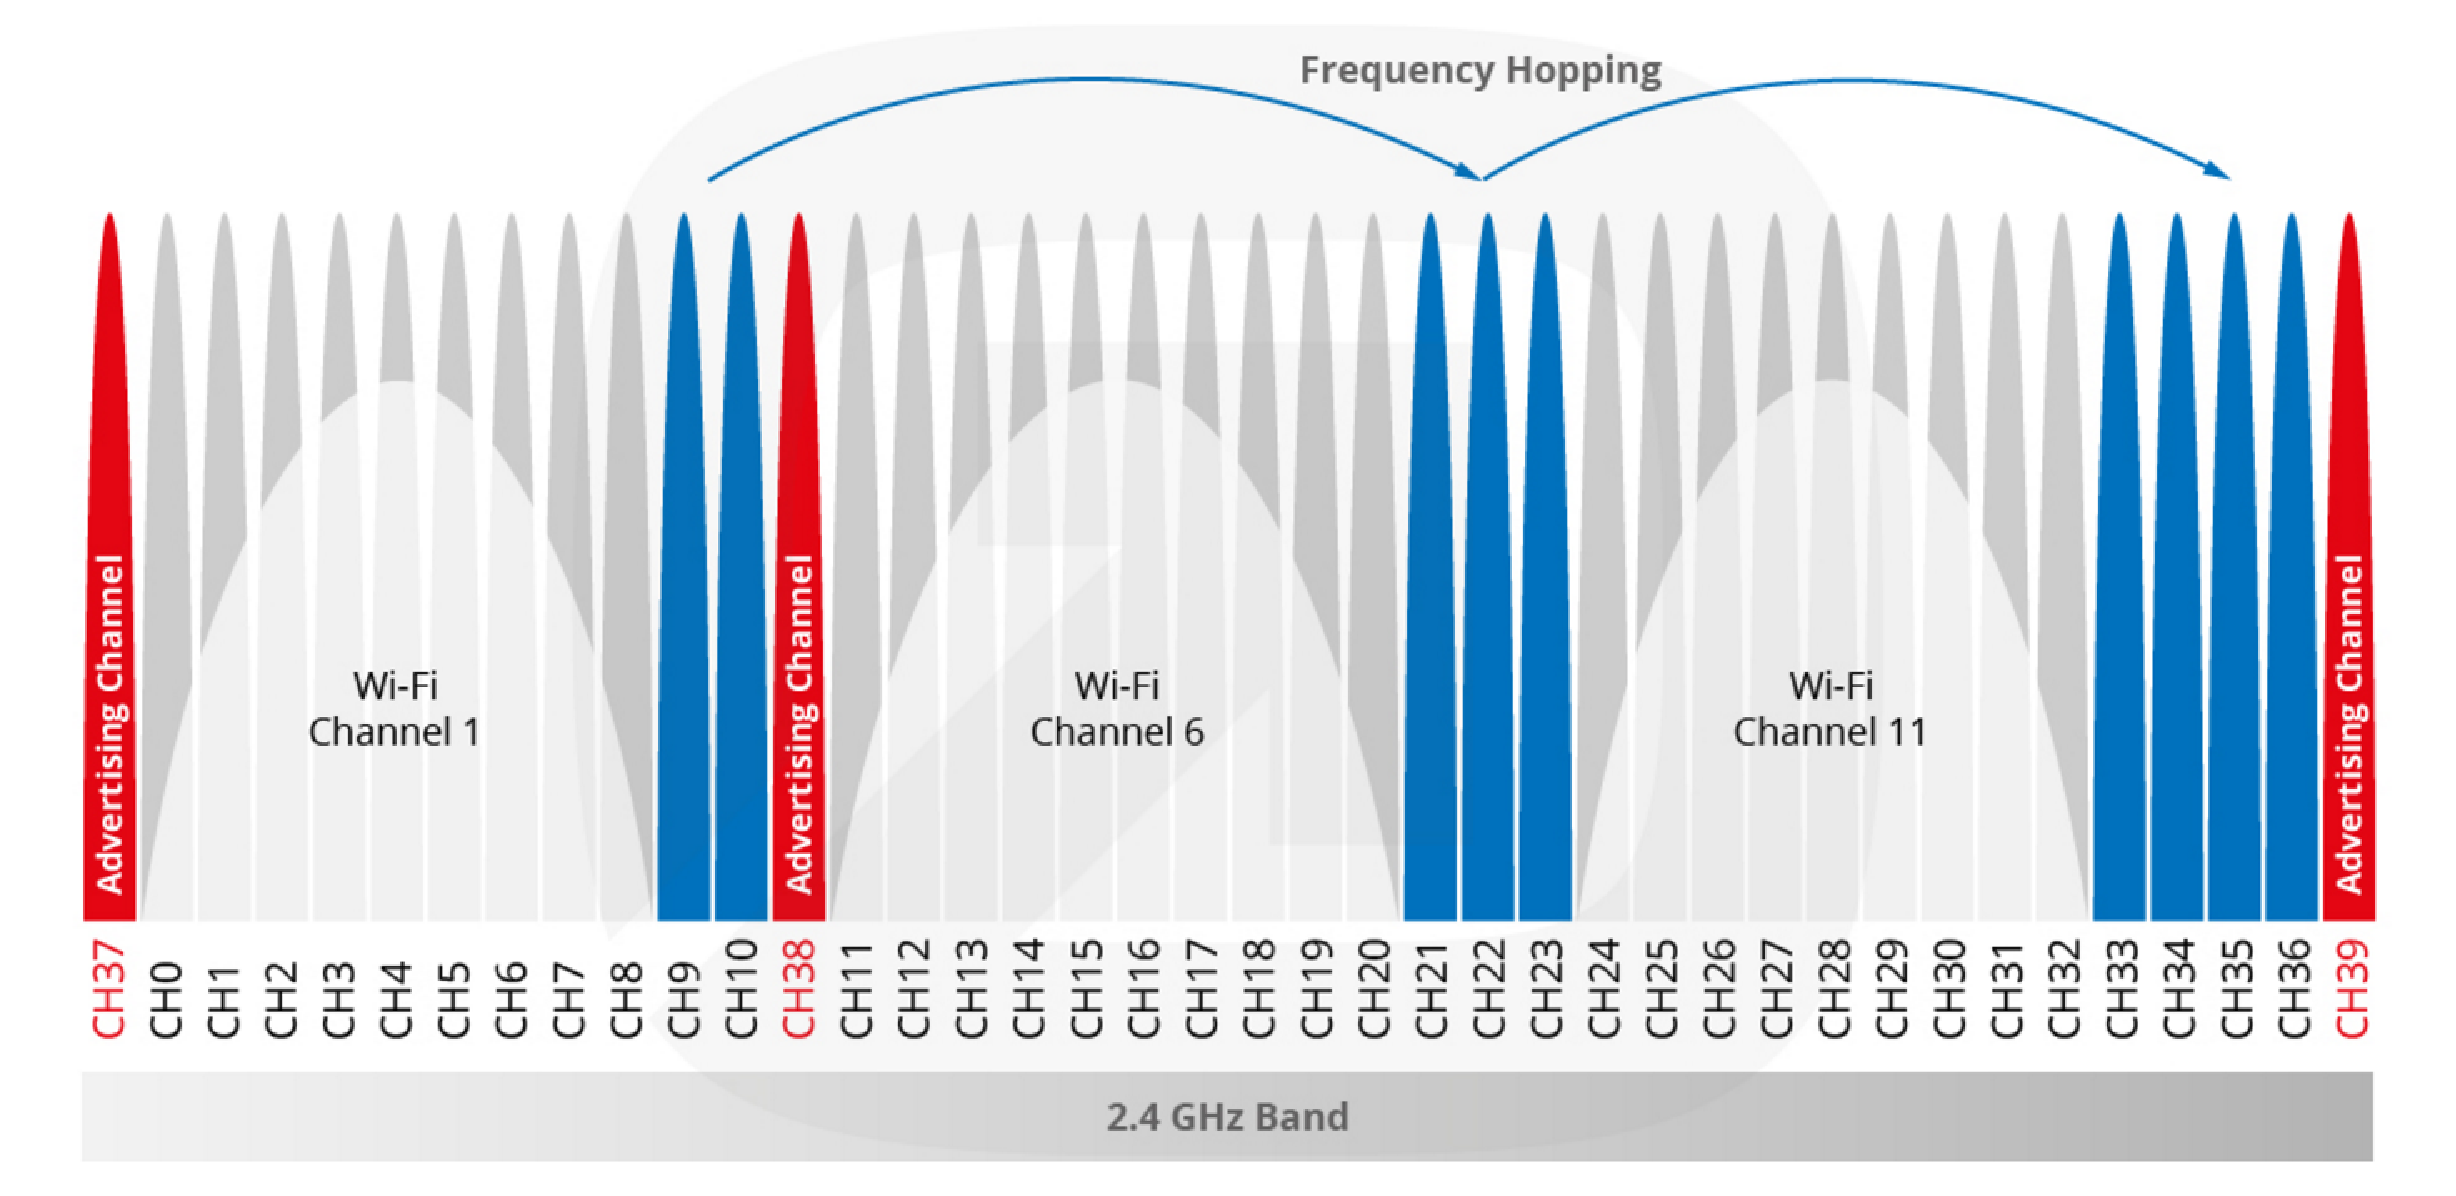
\includegraphics[width=0.7\textwidth]{./figures/channels.eps}
\end{center}
\begin{itemize}
\item Broadcasting data. The way to let know to other devices that you are present.
\item Transmit on all advertising cahnnel on each connection interval.
\item Connectable or non-conectable. 
\end{itemize}
}% =====================================   END FRAME   ==========================================

\frame{% ===============================   START FRAME   ================================================
\frametitle{Bluetooth LE Modes} 
\begin{center}
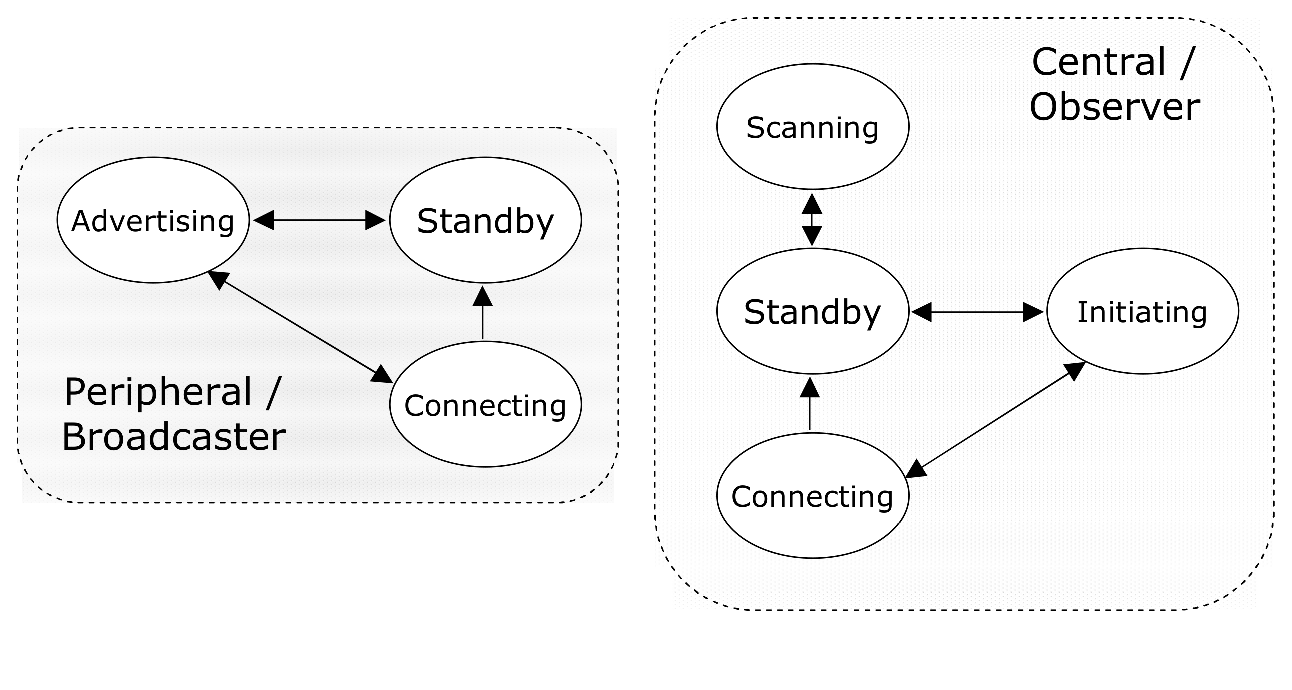
\includegraphics[width=0.7\textwidth]{./figures/conn1.eps}
\end{center}
}% =====================================   END FRAME   ==========================================

\frame{% ===============================   START FRAME   ================================================
\frametitle{Bluetooth LE Modes} 
\begin{center}
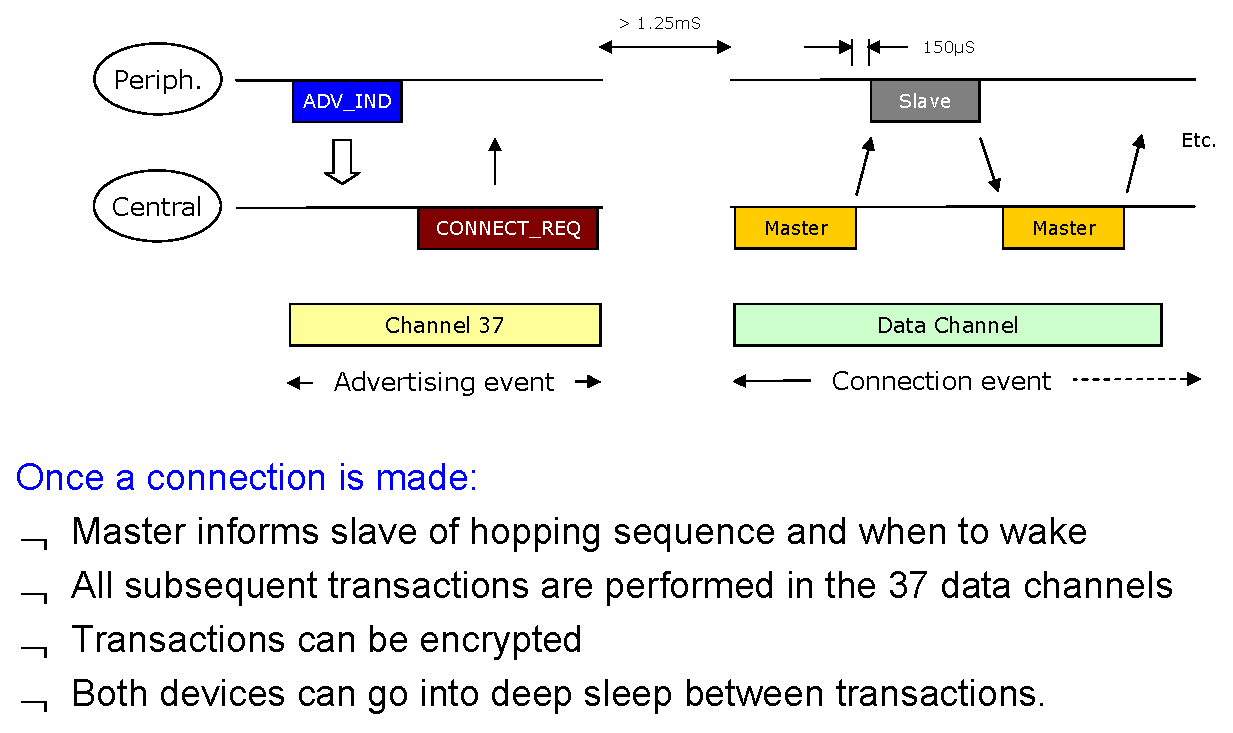
\includegraphics[width=0.7\textwidth]{./figures/conn2.eps}
\end{center}
}% =====================================   END FRAME   ==========================================


\frame{% ===============================   START FRAME   ================================================
\frametitle{Profile setup} 
\begin{center}
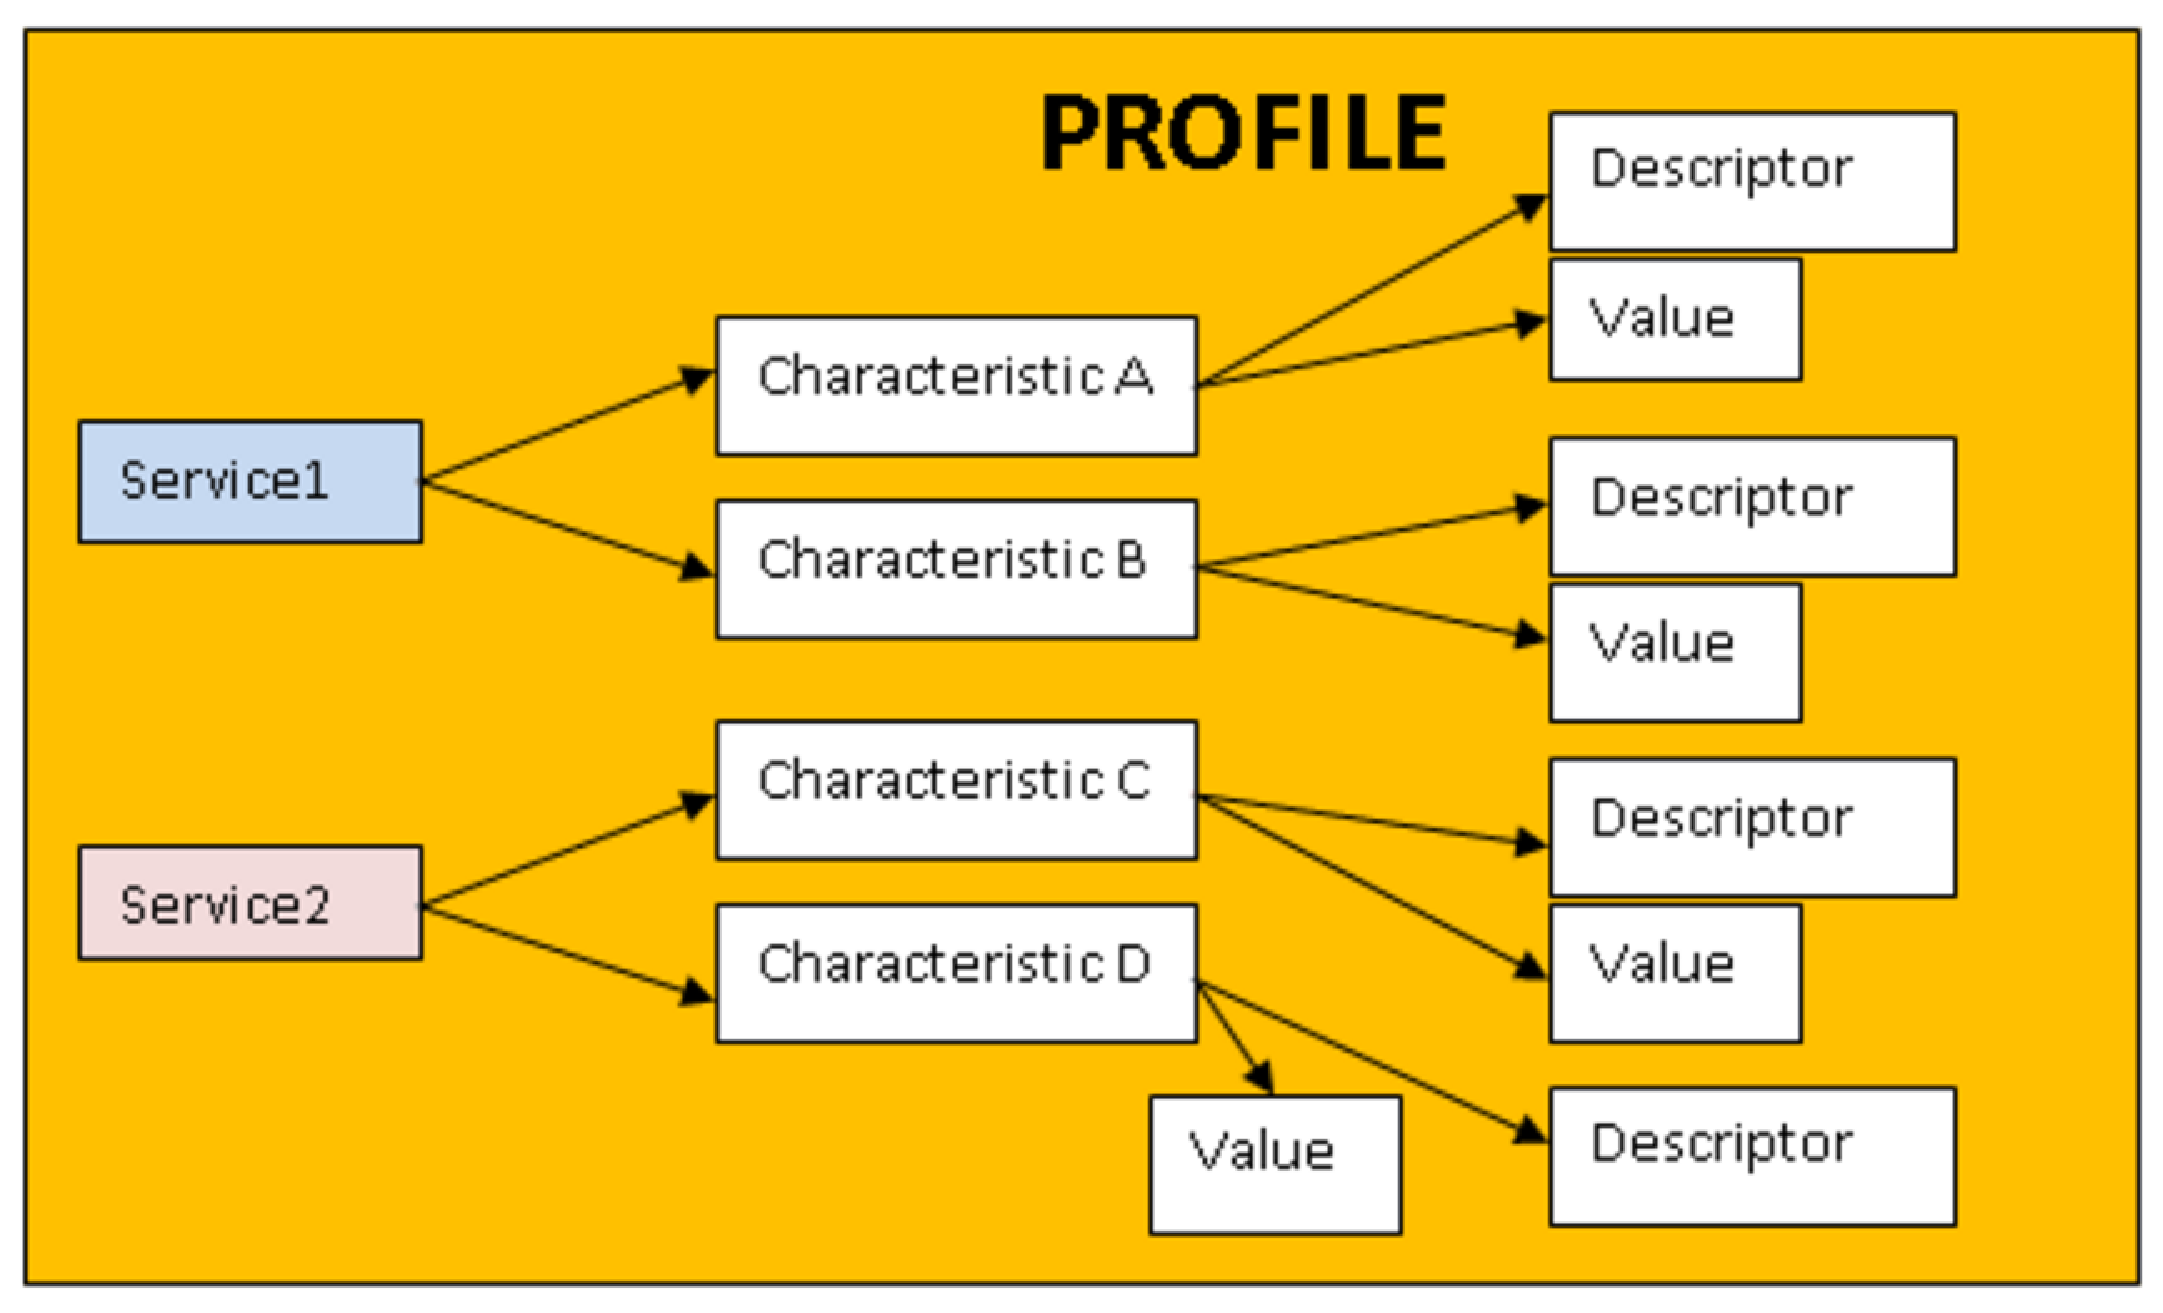
\includegraphics[width=0.5\textwidth]{./figures/profile.eps}
\end{center}

\begin{itemize}
\item \textbf{Profile:}
\begin{itemize}
\item In, BLE and application is considered as a Profile designed to exchange data. 
\item Overall application functionality
\end{itemize}
\item \textbf{Service:} Sub-functionality that consists of characteristics.
\item \textbf{Characteristics:} Performs its service functionality.  
\end{itemize}
}% =====================================   END FRAME   ==========================================

\frame{% ===============================   START FRAME   ================================================
\frametitle{Profile example, heart rate} 
\begin{center}
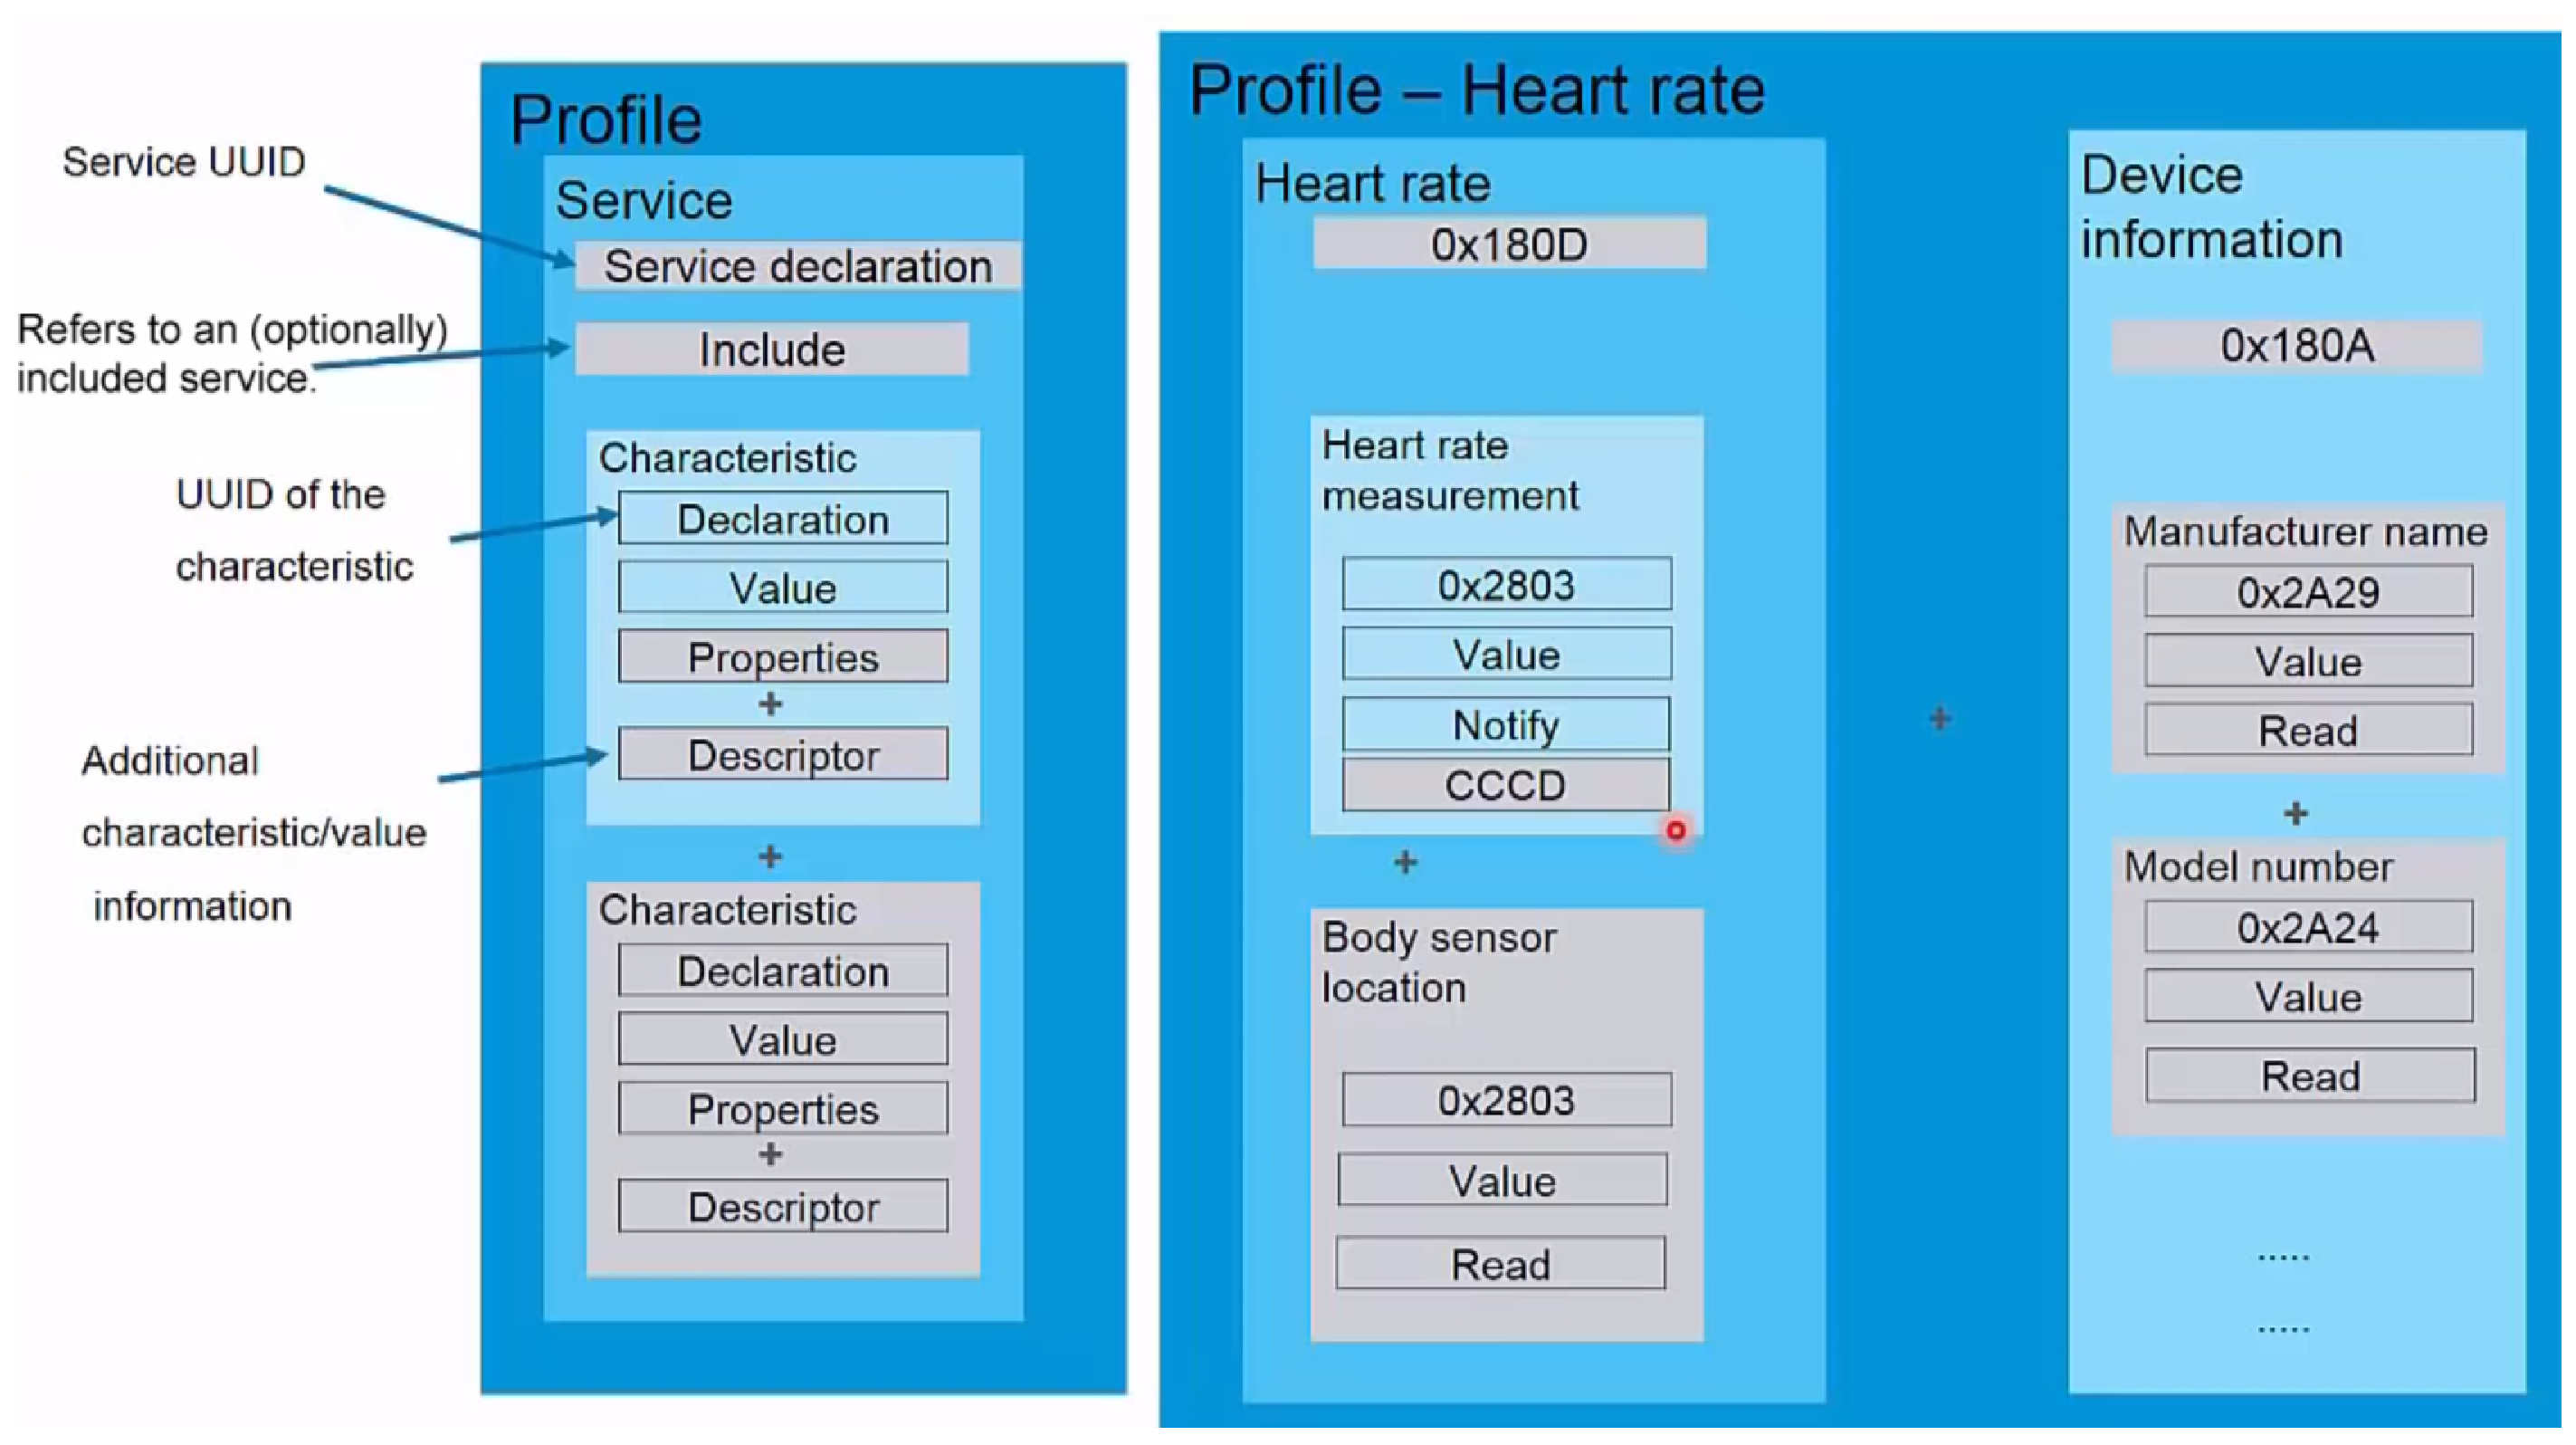
\includegraphics[width=0.85\textwidth]{./figures/profile2.eps}
\end{center}
}% =====================================   END FRAME   ==========================================



\frame{% ===============================   START FRAME   ================================================
\frametitle{Bluetooth Low Energy Power Consumption} 
\begin{center}
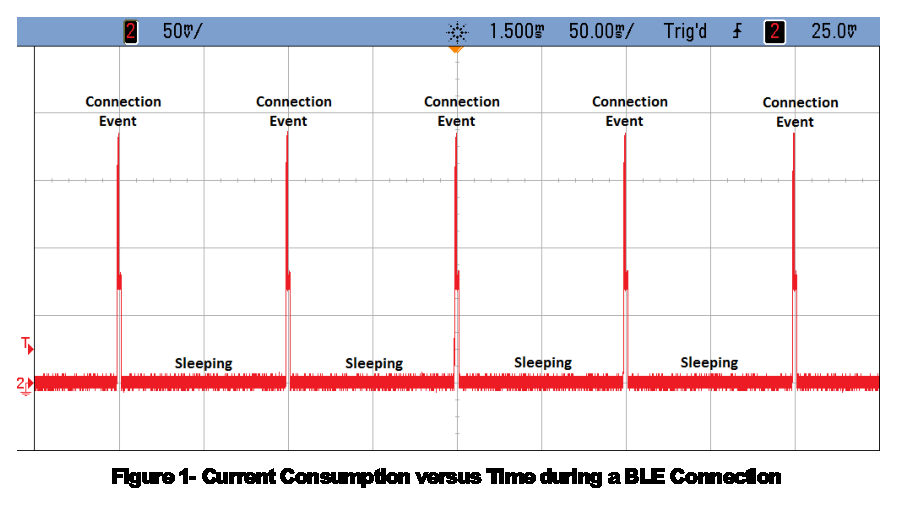
\includegraphics[width=0.5\textwidth]{./figures/ble1.eps}\footnote{{\tiny Texas Insturments, Measuring Bluetooth® Low Energy Power Consumption, Application Note AN092}}
\end{center}
\begin{itemize}
\item BLE stack will only be consuming current at the peak level while it is transmitting.
\item BLE device is transmitting only for a small percentage of the total time that the device is connected.
\end{itemize}
}% =====================================   END FRAME   ==========================================

\frame{% ===============================   START FRAME   ================================================
\frametitle{Bluetooth GAP (Generic Access Profile) roles} 
\begin{center}
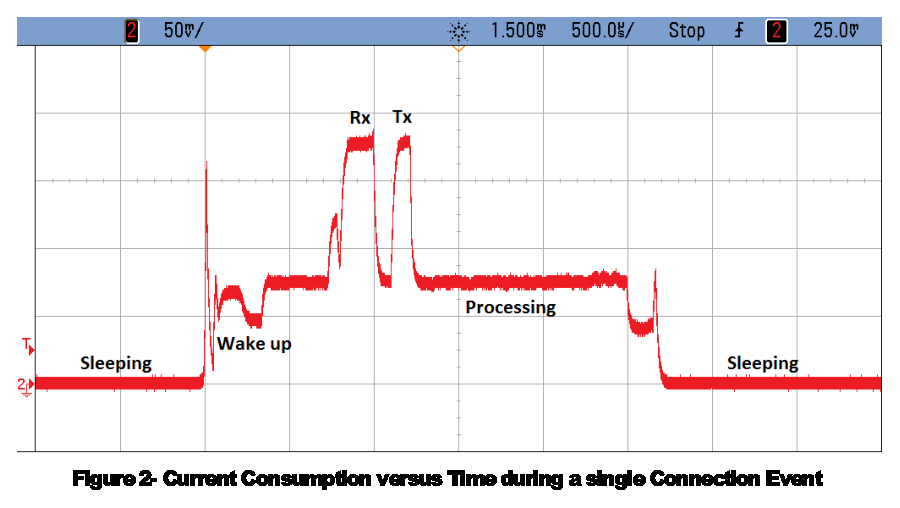
\includegraphics[width=0.85\textwidth]{./figures/ble2.eps}\footnote{{\tiny Texas Insturments, Measuring Bluetooth® Low Energy Power Consumption, Application Note AN092}}
\end{center}
}% =====================================   END FRAME   ==========================================


\frame{% ===============================   START FRAME   ================================================
\frametitle{Bluetooth GAP (Generic Access Profile) roles} 
\begin{center}
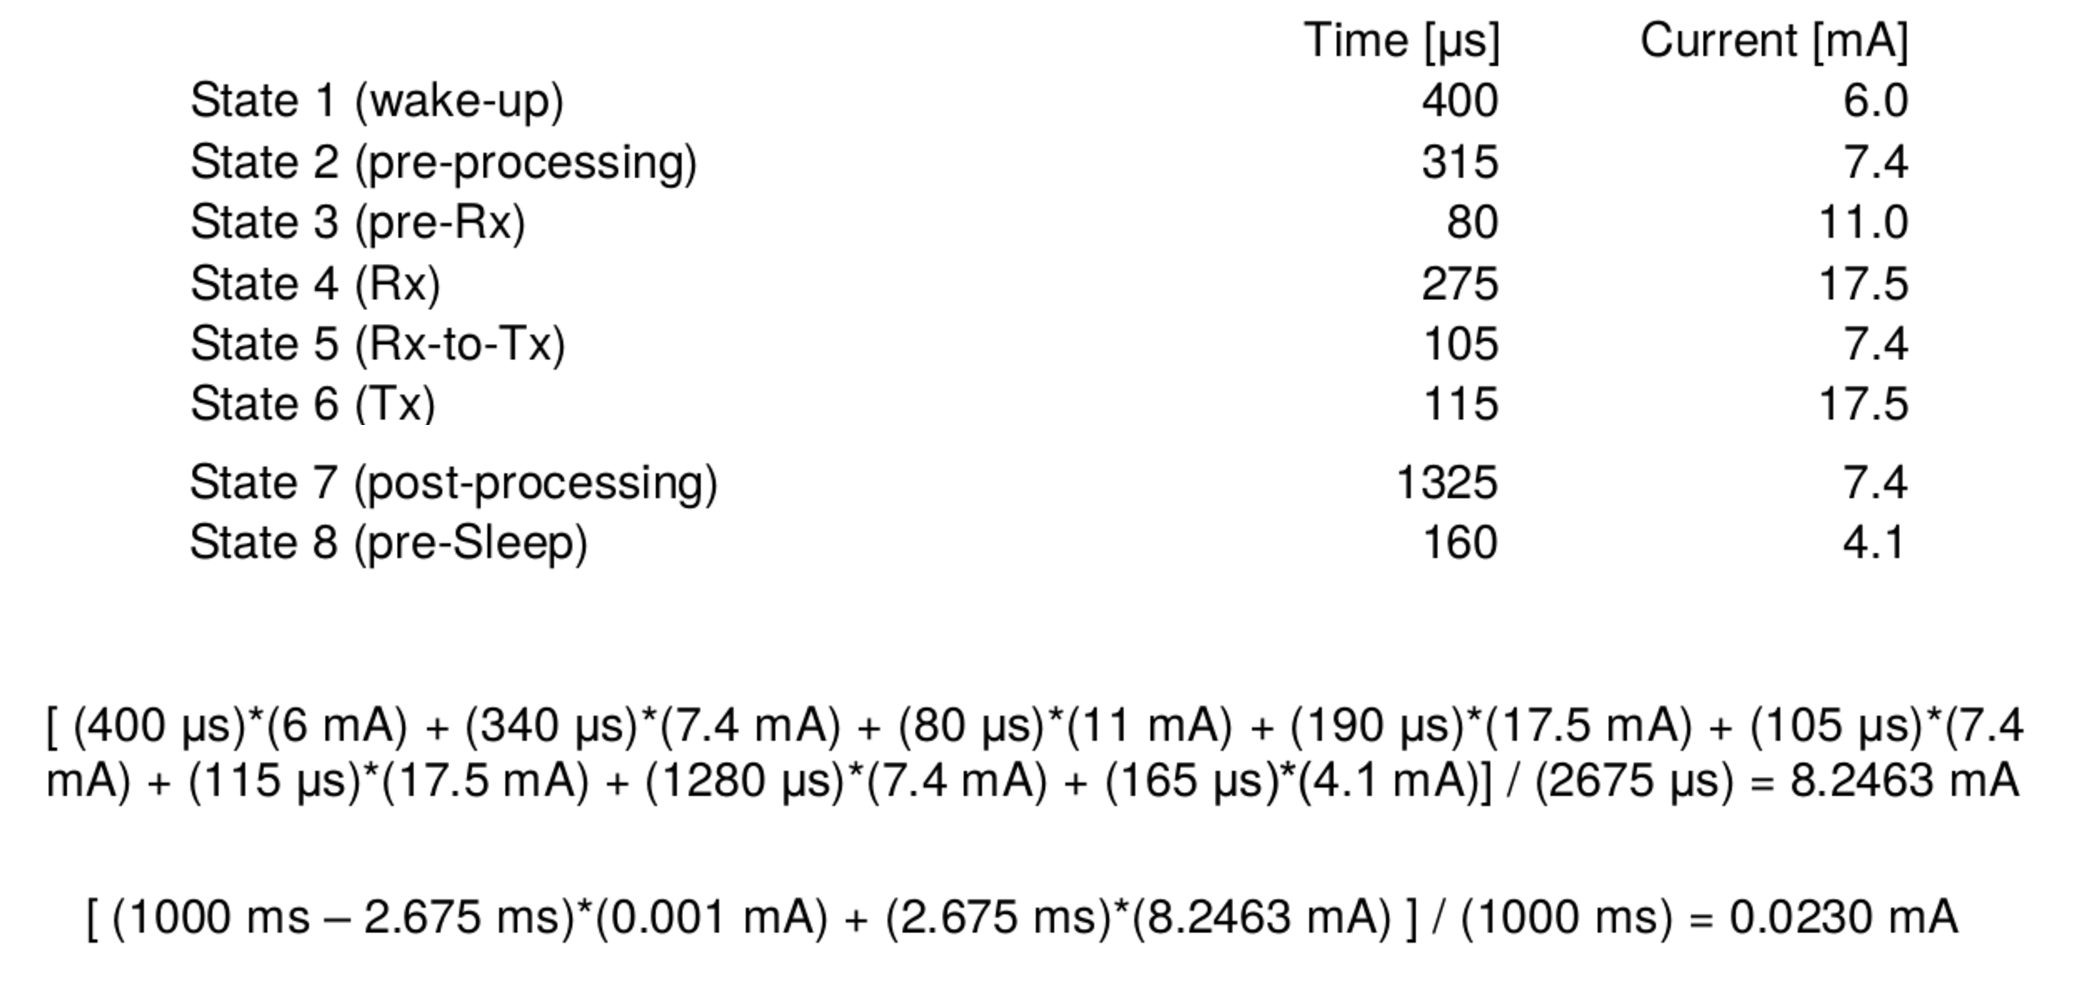
\includegraphics[width=0.7\textwidth]{./figures/ble3.eps}\footnote{{\tiny Texas Insturments, Measuring Bluetooth® Low Energy Power Consumption, Application Note AN092}}
\end{center}
}% =====================================   END FRAME   ==========================================



\frame{% ===============================   START FRAME   ================================================
\frametitle{Bluetooth GAP (Generic Access Profile) roles} 
\begin{center}
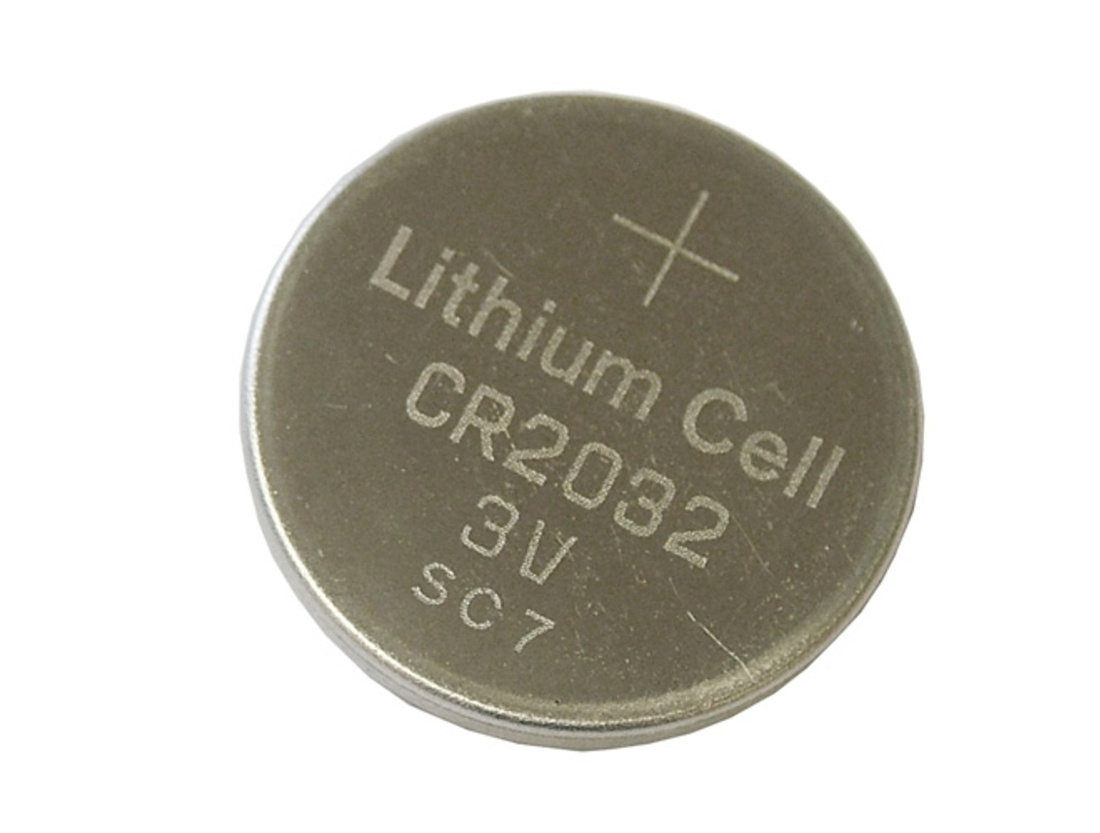
\includegraphics[width=0.35\textwidth]{./figures/cr2032.eps}
\end{center}
\begin{equation*}
(230mAh)/(0.023mA) = 10000 \text{ hours} = 416 \text{ days} = 1.14 \text{ years}
\end{equation*}
}% =====================================   END FRAME   ==========================================


\frame{% ===============================   START FRAME   ================================================
\frametitle{Bluetooth LE Layers} 
\begin{center}
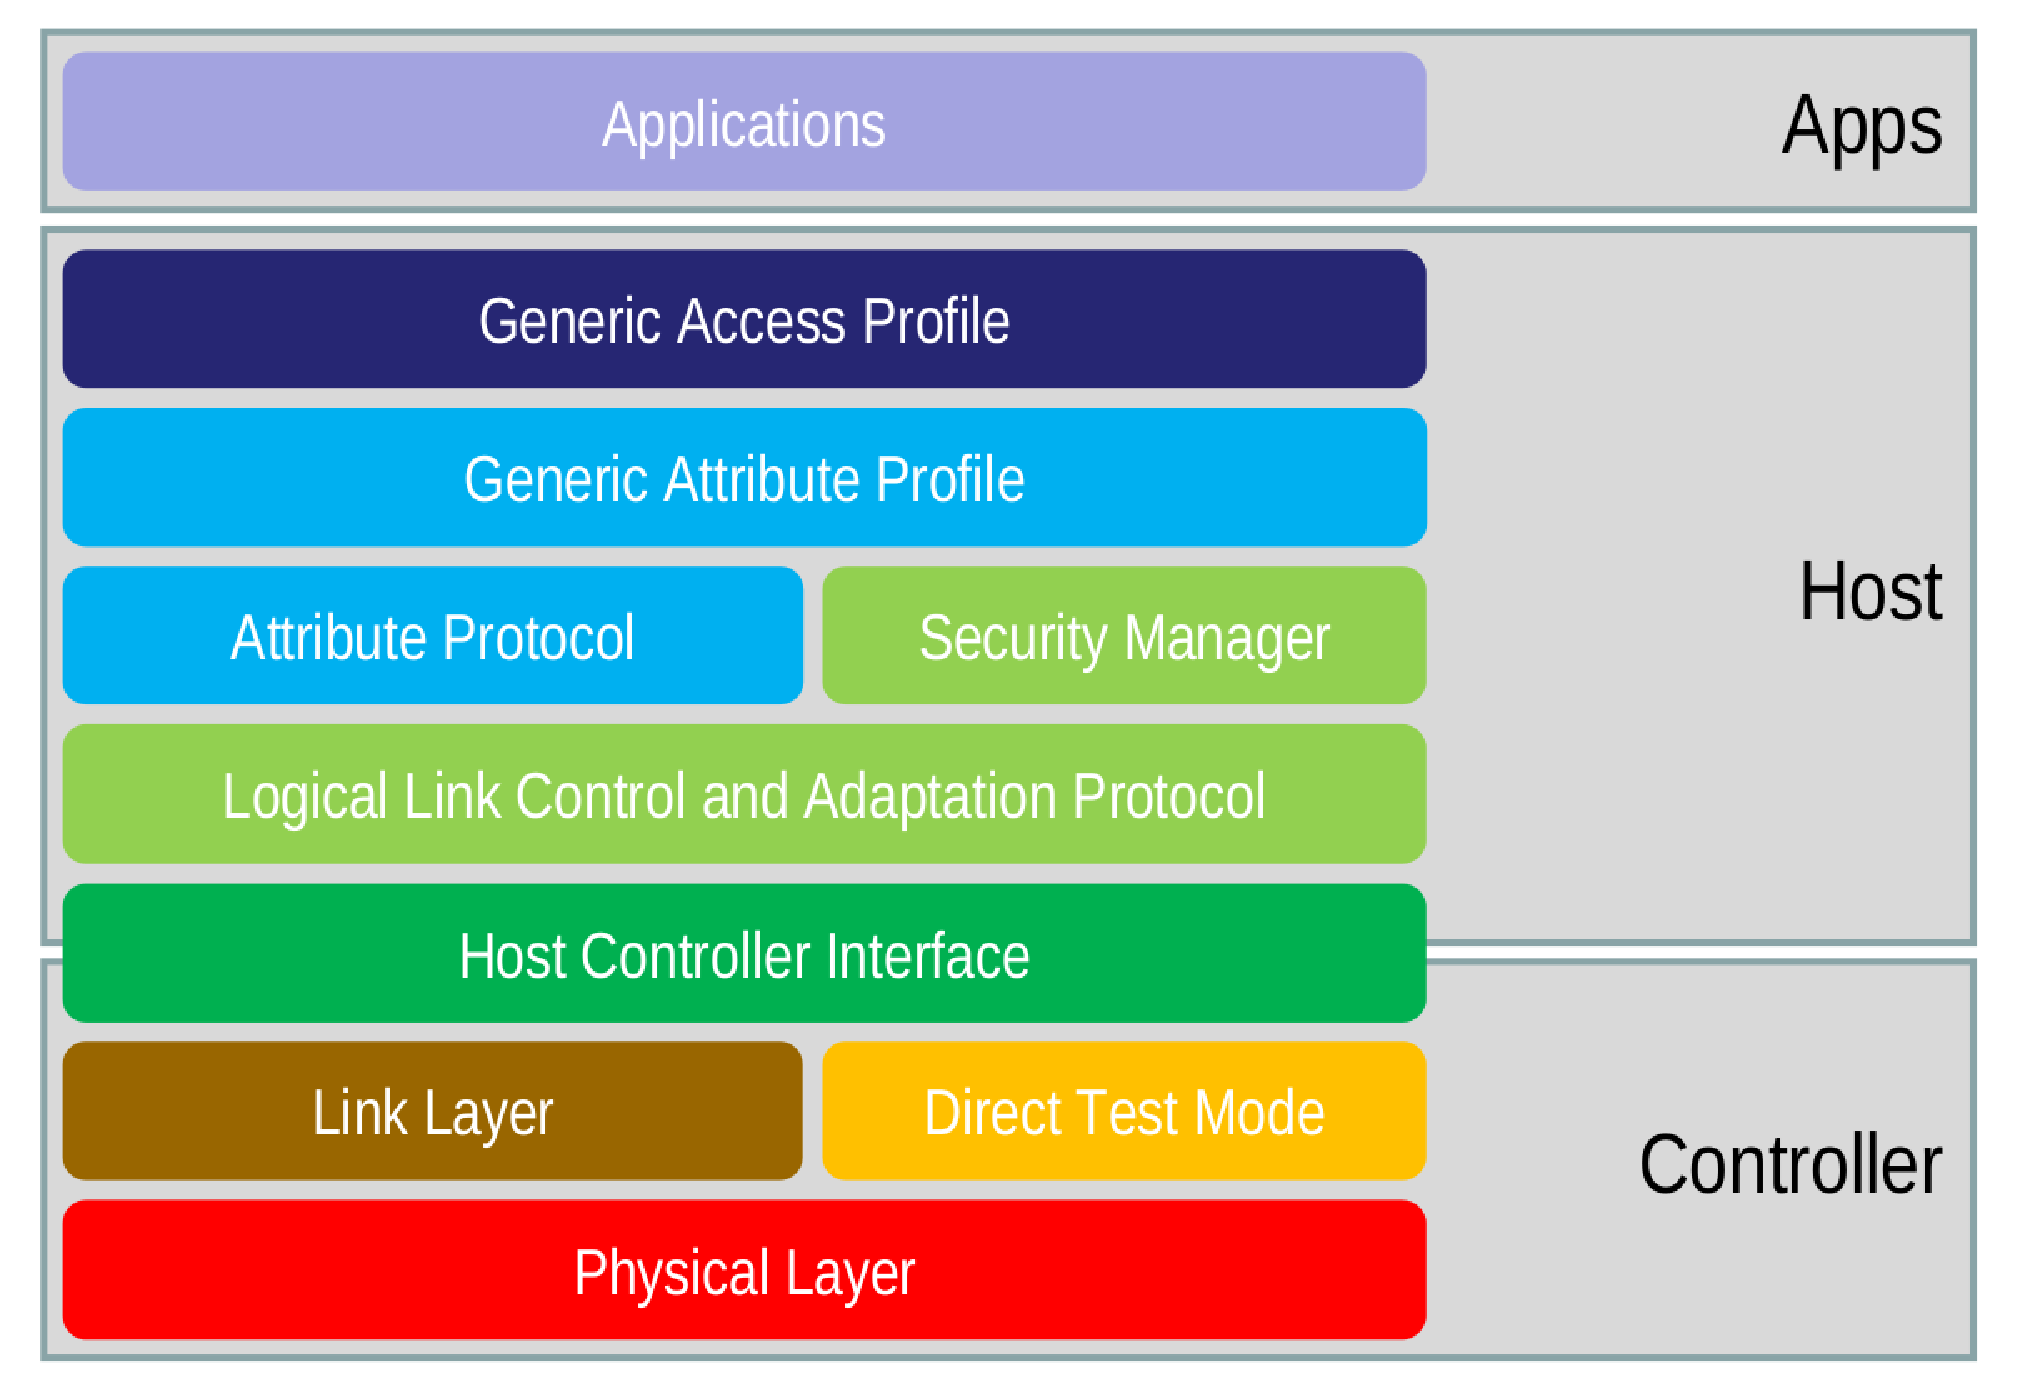
\includegraphics[width=0.7\textwidth]{./figures/layers.eps}
\end{center}
}% =====================================   END FRAME   ==========================================


\frame{% ===============================   START FRAME   ================================================
\frametitle{Bluetooth LE Layers} 
\begin{center}
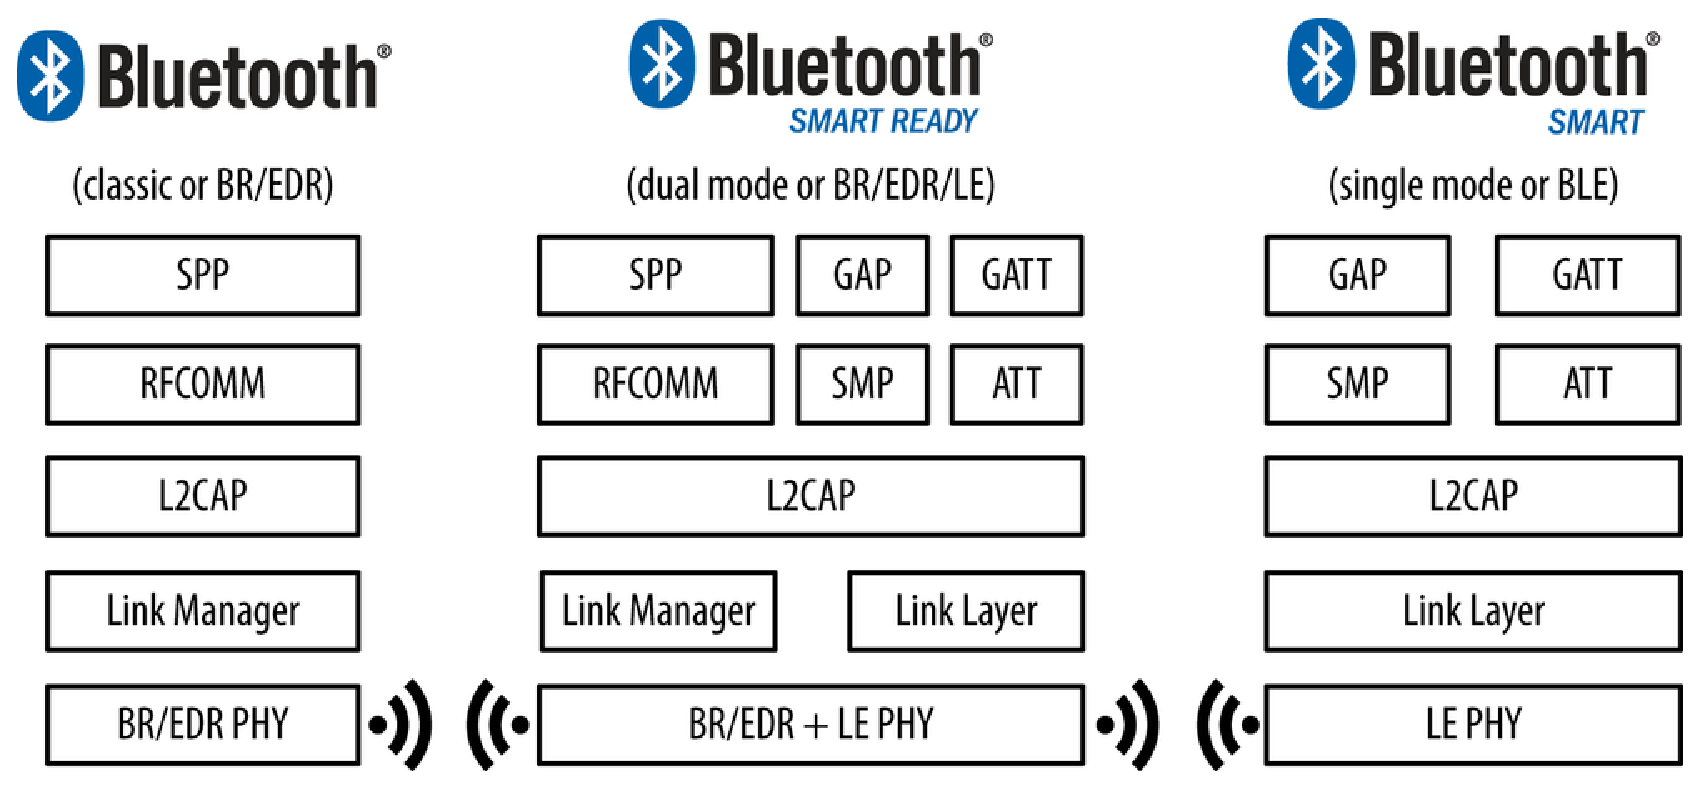
\includegraphics[width=0.75\textwidth]{./figures/bleComp.eps}
\end{center}
}% =====================================   END FRAME   ==========================================

\frame{% ===============================   START FRAME   ================================================
\frametitle{Bluetooth LE Modules} 
\begin{center}
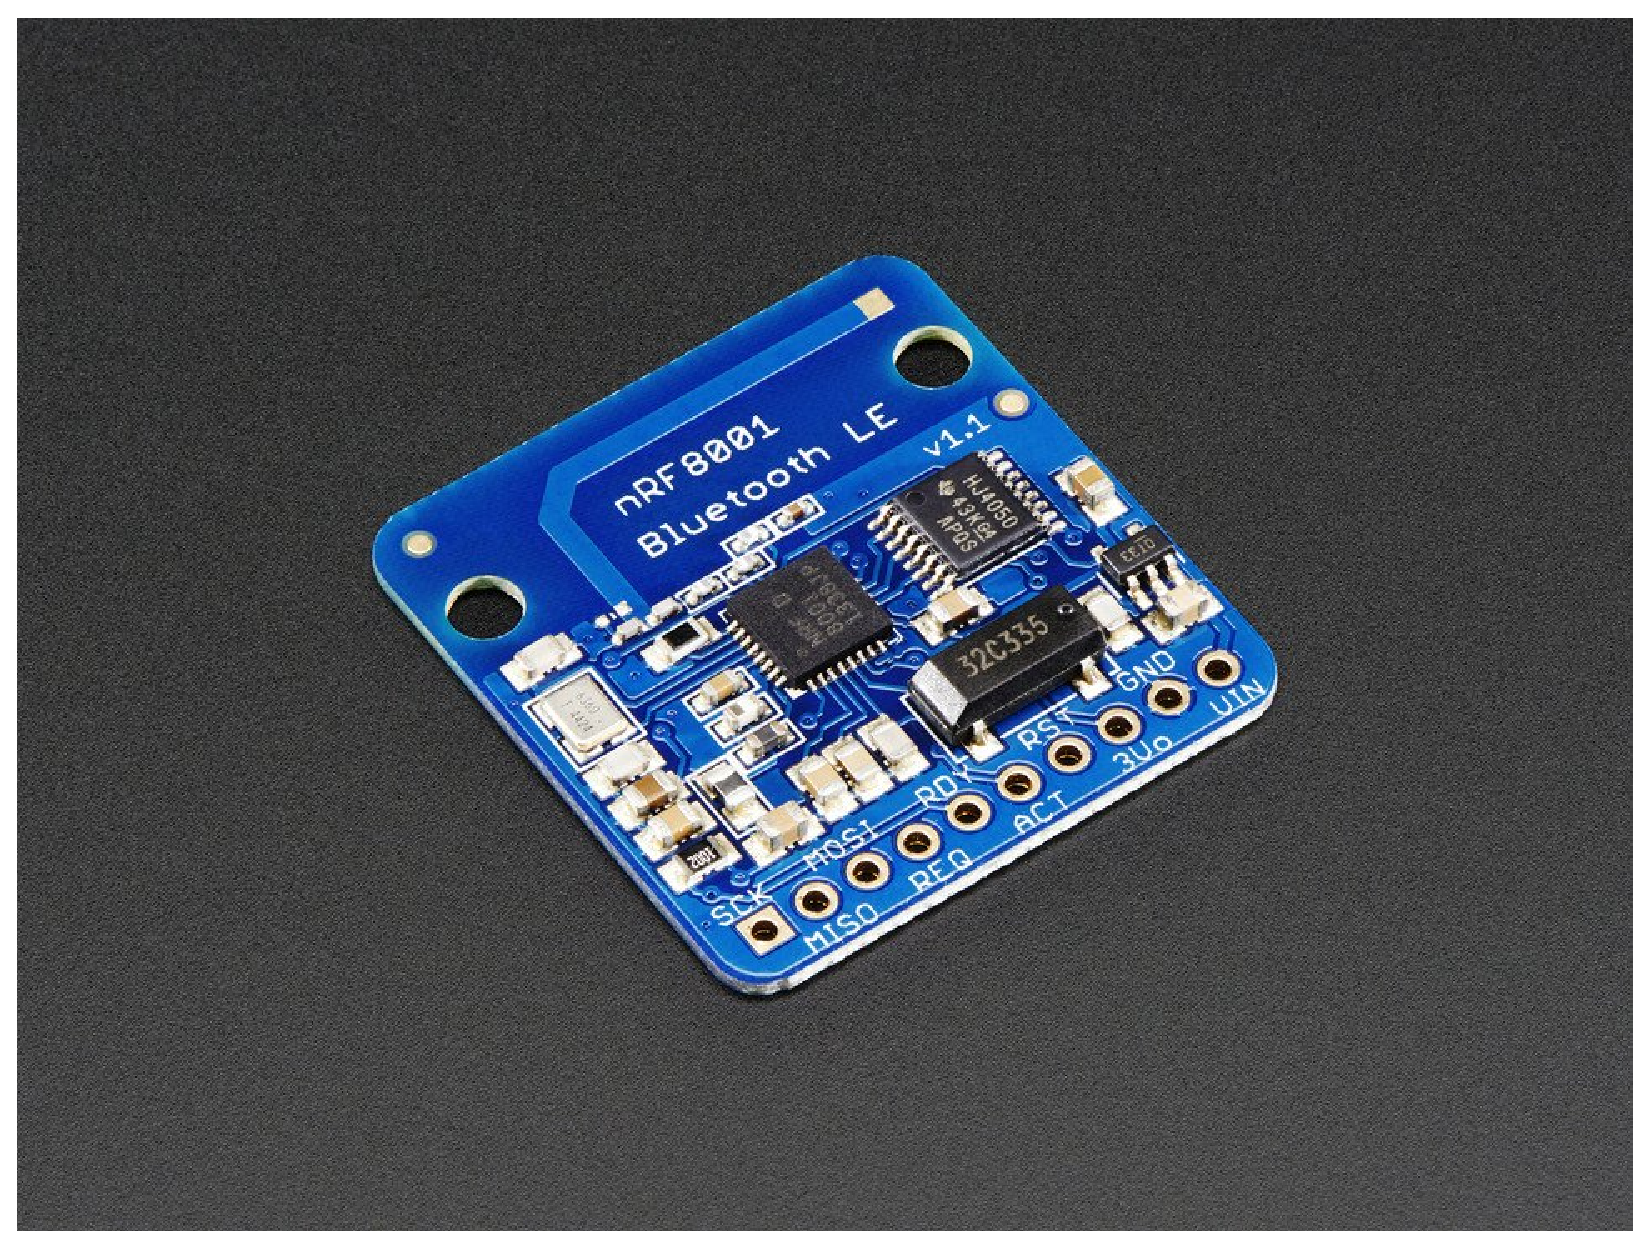
\includegraphics[width=0.75\textwidth]{./figures/nordig1.eps}
\end{center}
}% =====================================   END FRAME   ==========================================


\frame{% ===============================   START FRAME   ================================================
\frametitle{Bluetooth LE Modules} 
\begin{center}
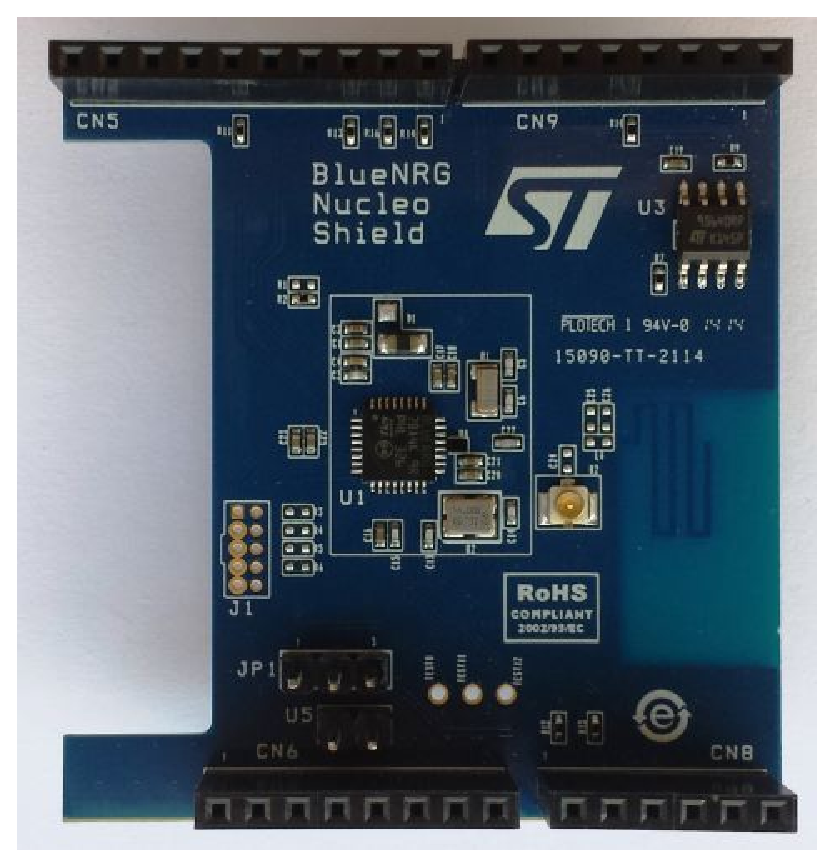
\includegraphics[width=0.5\textwidth]{./figures/xnucleo.eps}
\end{center}
}% =====================================   END FRAME   ==========================================


\frame{% ===============================   START FRAME   ================================================
\frametitle{Bluetooth LE Modules} 
\begin{center}
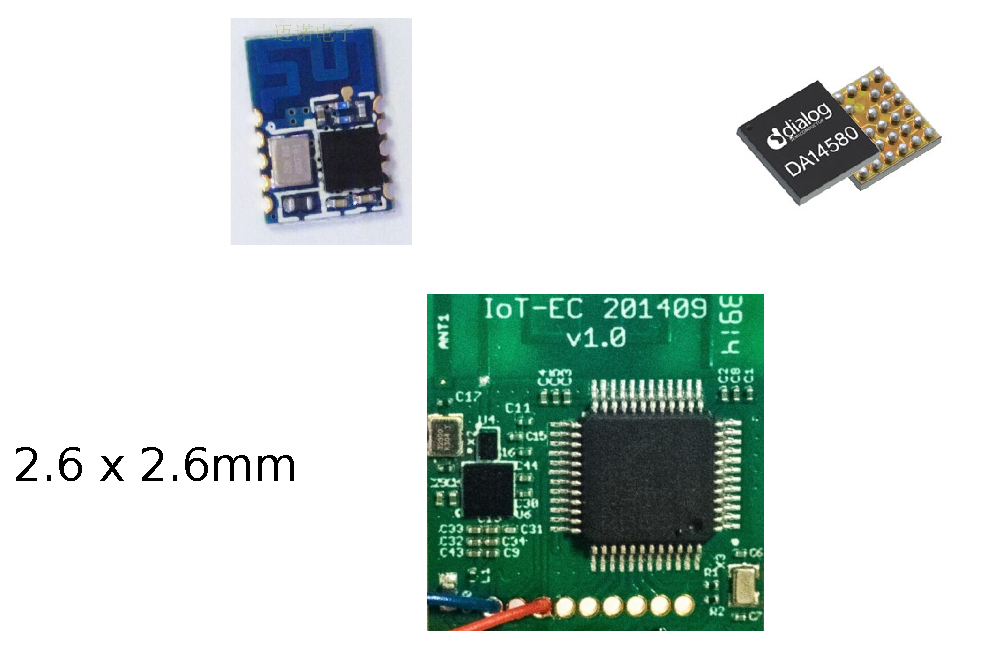
\includegraphics[width=0.5\textwidth]{./figures/board.eps}
\end{center}
}% =====================================   END FRAME   ==========================================


\frame{% ===============================   START FRAME   ================================================
\frametitle{Bluetooth LE Modules} 
\begin{center}
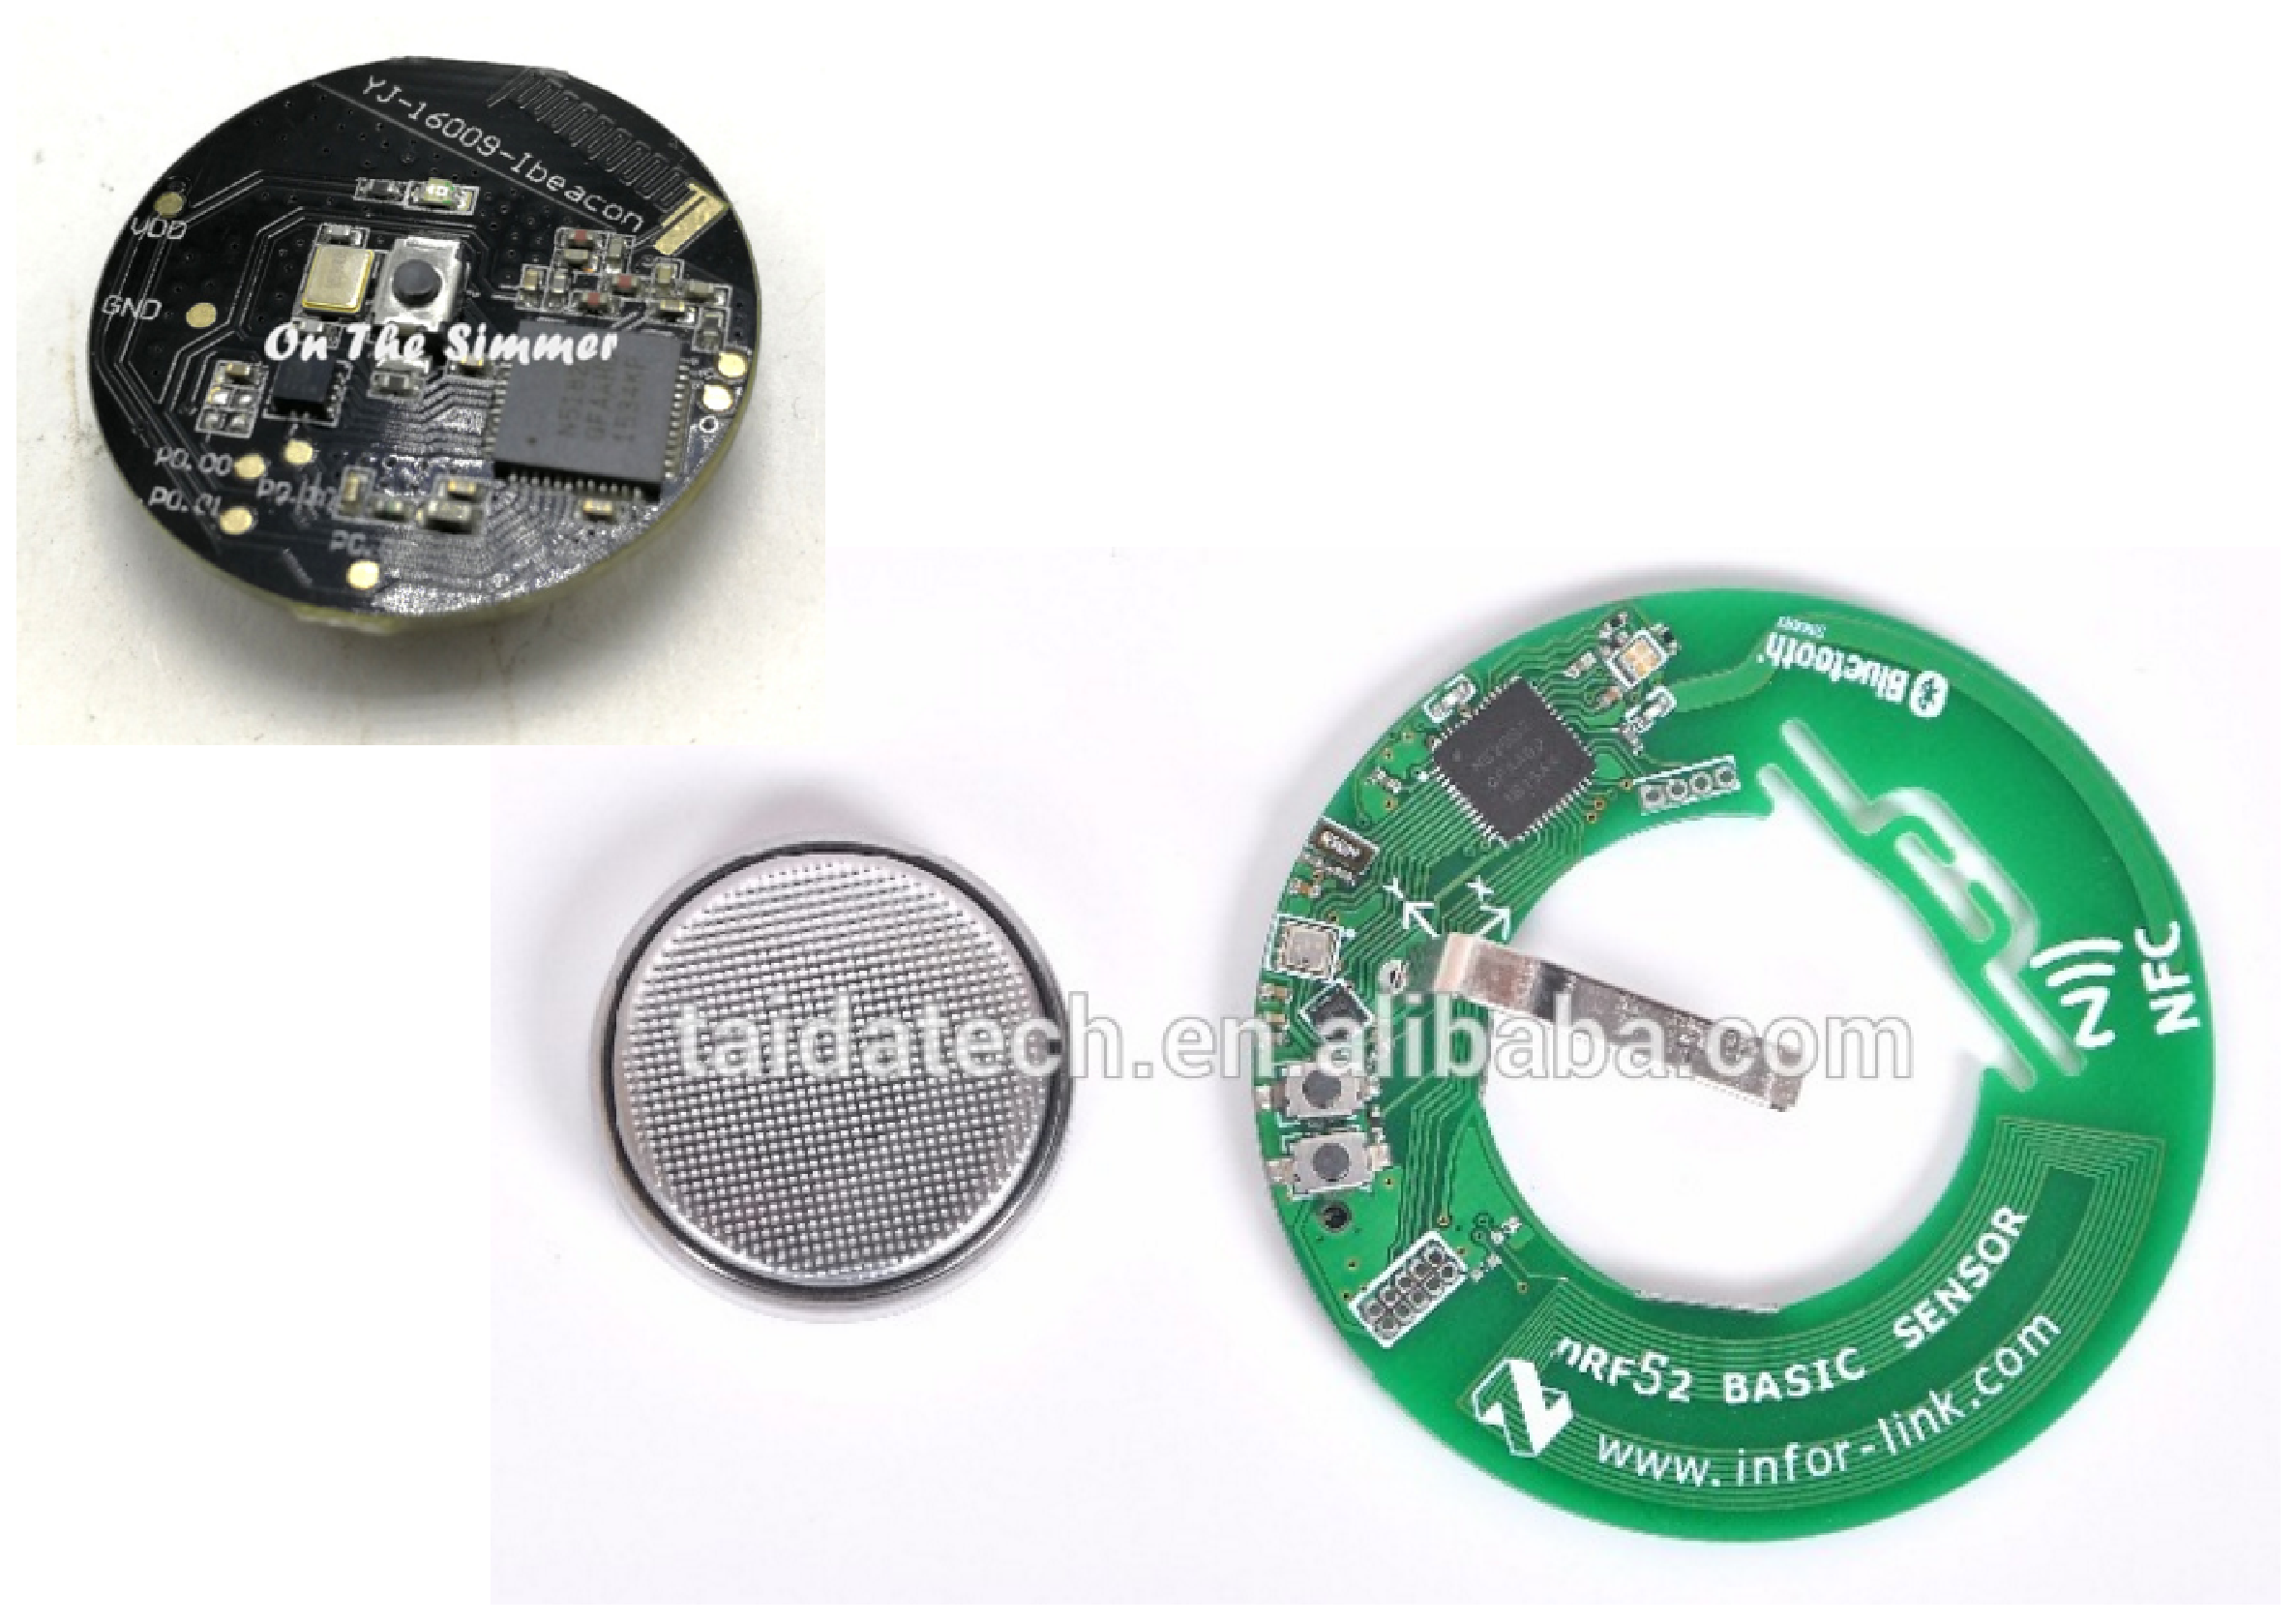
\includegraphics[width=.65\textwidth]{./figures/boards.eps}
\end{center}
}% =====================================   END FRAME   ==========================================


\end{document}